\documentclass[../../main.tex]{subfiles}
\graphicspath{{../../image/}{../../figure/}}
\begin{document}

\section{黏性激波剖面}\label{section:ch08-黏性激波剖面}

使用消失黏性方法来识别双曲守恒律系统容许弱解的思想，是在\cref{section:ch04-消失黏性方法}中引入的。在一维空间的当下设定中，对系统\eqref{align:ch08-守恒律一维}，方程\eqref{align:ch04-黏性组} 蜕化为
\begin{align}
\partial_t U(x,t)+\partial_x F(U(x,t))=\mu\,\partial_x\big[B(U(x,t))\partial_x U(x,t)\big].
\label{align:ch08-黏性方程}
\end{align}

如\cref{section:ch04-消失黏性方法}已解释，$n\times n$ 矩阵值函数 $B$ 的选取可由系统的物理背景提示，也可能只是分析的人为产物。例如考虑耗散系统
\begin{align}
\partial_t u+\partial_x f(u)=\mu\,\partial_x^2 u,
\label{align:ch08-标量黏性}
\end{align}
\begin{align}
\begin{cases}
\partial_t u-\partial_x v=0\\
\partial_t v-\partial_x\sigma(u)=\mu\,\partial_x(u^{-1}\partial_x v),
\end{cases}
\label{align:ch08-弹性黏性}
\end{align}
\begin{align}
\begin{cases}
\partial_t u+\partial_x\big[(u^2+v^2)u\big]=\mu\,\partial_x^2 u\\
\partial_t v+\partial_x\big[(u^2+v^2)v\big]=\mu\,\partial_x^2 v,
\end{cases}
\label{align:ch08-模型黏性}
\end{align}
它们分别关联于双曲系统\eqref{align:ch07-标量守恒律}、\eqref{align:ch07-p系统}、\eqref{align:ch07-脐点模型}。就\eqref{align:ch07-p系统} 被解释为等熵气体动力学系统而言，\eqref{align:ch08-弹性黏性} 中黏性的选取是由物理决定的\footnote{与\eqref{align:ch04-NS} 比较。变黏性系数 $\mu u^{-1}$ 的采用，是为了在通常进行测量的空间设定中黏性为常数 $\mu$。当然，这仅当 $u>0$ 时才有意义。}。另一方面，在\eqref{align:ch08-标量黏性} 与\eqref{align:ch08-模型黏性} 中，黏性是人为的。

与熵准则相反，由消失黏性准则判定弱解的容许性是否仅在激波集层面决定，这一点完全不清楚。然而，姑且把这一前提视为当然，那么只需在形如
\begin{align}
U(x,t)=
\begin{cases}
U_-,&x<st\\
U_+,&x>st,
\end{cases}
\label{align:ch08-间断}
\end{align}
的解的语境中检验容许性即可，即一个速度为常数 $s$、在左侧连接常状态 $U_-$、在右侧连接常状态 $U_+$ 的激波。可以设想，函数\eqref{align:ch08-间断} 当 $\mu\downarrow0$ 时可由\eqref{align:ch08-黏性方程} 的一族行波形式解 $U_\mu$ 逼近，即单变量 $x-st$ 的函数。利用\eqref{align:ch08-黏性方程} 中的伸缩，我们寻求形如
\begin{align}
U_\mu(x,t)=V\!\left(\frac{x-st}{\mu}\right).
\label{align:ch08-行波形式}
\end{align}
的解族。

将\eqref{align:ch08-行波形式} 代入\eqref{align:ch08-黏性方程}，推得 $V$ 应满足常微分方程
\begin{align}
\big[B(V(\tau))\dot V(\tau)\big]^{\cdot}=\dot F(V(\tau))-s\dot V(\tau),
\label{align:ch08-行波ode}
\end{align}
其中圆点表示关于 $\tau=(x-st)/\mu$ 的导数。我们感兴趣的是在 $V=U_-$ 处 $\dot V$ 为零的解，于是将\eqref{align:ch08-行波ode} 关于 $\tau$ 积分一次，得
\begin{align}
B(V)\dot V=F(V)-F(U_-)-s[V-U_-].
\label{align:ch08-剖面ode}
\end{align}
注意\eqref{align:ch08-剖面ode} 的右端在可由速度 $s$ 的激波连到 $U_-$ 的 $V$ 集上为零。该集特别包含状态 $U_+$。因此 $U_-$ 与 $U_+$ 都是\eqref{align:ch08-剖面ode} 的平衡点。

连接一条激波左状态 $U_-$ 与右状态 $U_+$ 的\emph{黏性激波剖面}，是一条端点为 $U_-$、$U_+$ 的光滑弧，它是微分方程\eqref{align:ch08-剖面ode} 的不变集，并且在弧上任何非平衡点处，流的方向是从 $U_-$ 到 $U_+$。

将 $U_-$（左）连接到 $U_+$（右）的激波，当且仅当 $U_-$ 可由一条黏性激波剖面连到 $U_+$ 时，称为满足\emph{黏性激波容许性准则}。

确定黏性激波剖面之所以重要，不仅因为它们阐明了容许性问题，还因为它们（至少在矩阵 $B$ 受物理驱动时）提供了关于激波所刻画的尖锐跃迁性质——即所谓激波结构——的信息。确实，\eqref{align:ch08-行波形式} 中涉及的坐标伸缩当 $\mu\downarrow0$ 时，好比让人在显微镜下观察激波。

一般而言，黏性激波剖面可包含有限或无穷多个平衡点，其中任意两个相邻平衡点由\eqref{align:ch08-剖面ode} 的轨道相连。作为一个极端情形，注意当连接 $U_-$ 与 $U_+$ 的激波是关联于线性退化特征族的接触间断时，由\cref{theorem:ch08-线性退化激波曲线}，连接 $U_-$ 与 $U_+$ 的激波曲线上每一点都是\eqref{align:ch08-剖面ode} 的平衡点，因而激波曲线本身就充当黏性激波剖面。我们现考虑更典型的情形：$U_-$ 与 $U_+$ 是黏性激波剖面上仅有的平衡点，于是 $U_-$ 是\eqref{align:ch08-剖面ode} 某条轨道的 $\alpha$-极限集，$U_+$ 是其 $\omega$-极限集。

为说明并与\hyperref[section:ch08-lax容许性准则]{8.3 节}的讨论建立联系，设连接 $U_-$（左）与 $U_+$（右）的激波速度 $s$ 满足\eqref{align:ch08-lax谱条件}。为确定起见，取恒等矩阵为黏性矩阵 $B$，于是黏性激波剖面将是系统
\begin{align}
\dot V=F(V)-F(U_-)-s[V-U_-].
\label{align:ch08-id剖面}
\end{align}
的轨道。回顾\eqref{align:ch08-rh} 并在 $U_\pm$ 附近线性化\eqref{align:ch08-id剖面}，得
\begin{align}
\dot W=[\mathrm{D}F(U_\pm)-sI]W.
\label{align:ch08-线性化}
\end{align}
矩阵 $\mathrm{D}F(U_-)-sI$ 的特征值为 $\lambda_1(U_-)-s,\cdots,\lambda_n(U_-)-s$，由\eqref{align:ch08-lax谱条件}，前 $i-1$ 个为负、其余 $n-i+1$ 个为正。类似地，矩阵 $\mathrm{D}F(U_+)-sI$ 的特征值 $\lambda_1(U_+)-s,\cdots,\lambda_n(U_+)-s$ 中前 $j$ 个为负、其余 $n-j$ 个为正。由此可知 $U_-$ 与 $U_+$ 是\eqref{align:ch08-id剖面} 的局部孤立平衡点。进而，在 $U_-$ 的某个邻域内，任何 $\alpha$-极限集为 $U_-$ 的\eqref{align:ch08-id剖面} 轨道都驻留于不稳定流形 $\mathscr U$ 上，其维数为 $n-i+1$，并在 $U_-$ 处切于由特征向量 $R_i(U_-),\cdots,R_n(U_-)$ 张成的超平面。类似地，在 $U_+$ 的某个邻域内，任何 $\omega$-极限集为 $U_+$ 的轨道驻留于稳定流形 $\mathscr S$ 上，其维数为 $j$，并在 $U_+$ 处切于由特征向量 $R_1(U_+),\cdots,R_j(U_+)$ 张成的超平面。设激波强度与这一局部结构相称，于是黏性激波剖面是位于 $\mathscr U$ 与 $\mathscr S$ 交上的轨道。

对压缩激波（即 $i=j$），$\dim\mathscr U+\dim\mathscr S=n+1$，故 $\mathscr U$ 与 $\mathscr S$ 横截相交成一条曲线，它是连接 $U_-$ 与 $U_+$ 的唯一黏性激波剖面。进而，该剖面是\emph{结构稳定的}，即在 $U_-$、$U_+$ 与流函数 $F$ 的小扰动下稳定。图\ref{figure:ch08-三模式} (a) 描绘了 $n=2$、$i=j=1$ 的此类模式：不稳定结点 $U_-$ 以一条唯一的、结构稳定的黏性激波剖面连接到鞍点 $U_+$。图\ref{figure:ch08-二三流形} 描绘了 $n=3$、$i=j=2$ 的构型：二维不稳定流形 $\mathscr U$ 与二维稳定流形 $\mathscr S$ 横截相交，形成连接 $U_-$ 与 $U_+$ 的唯一、结构稳定的黏性激波剖面。

\begin{figure}[ht]
\centering
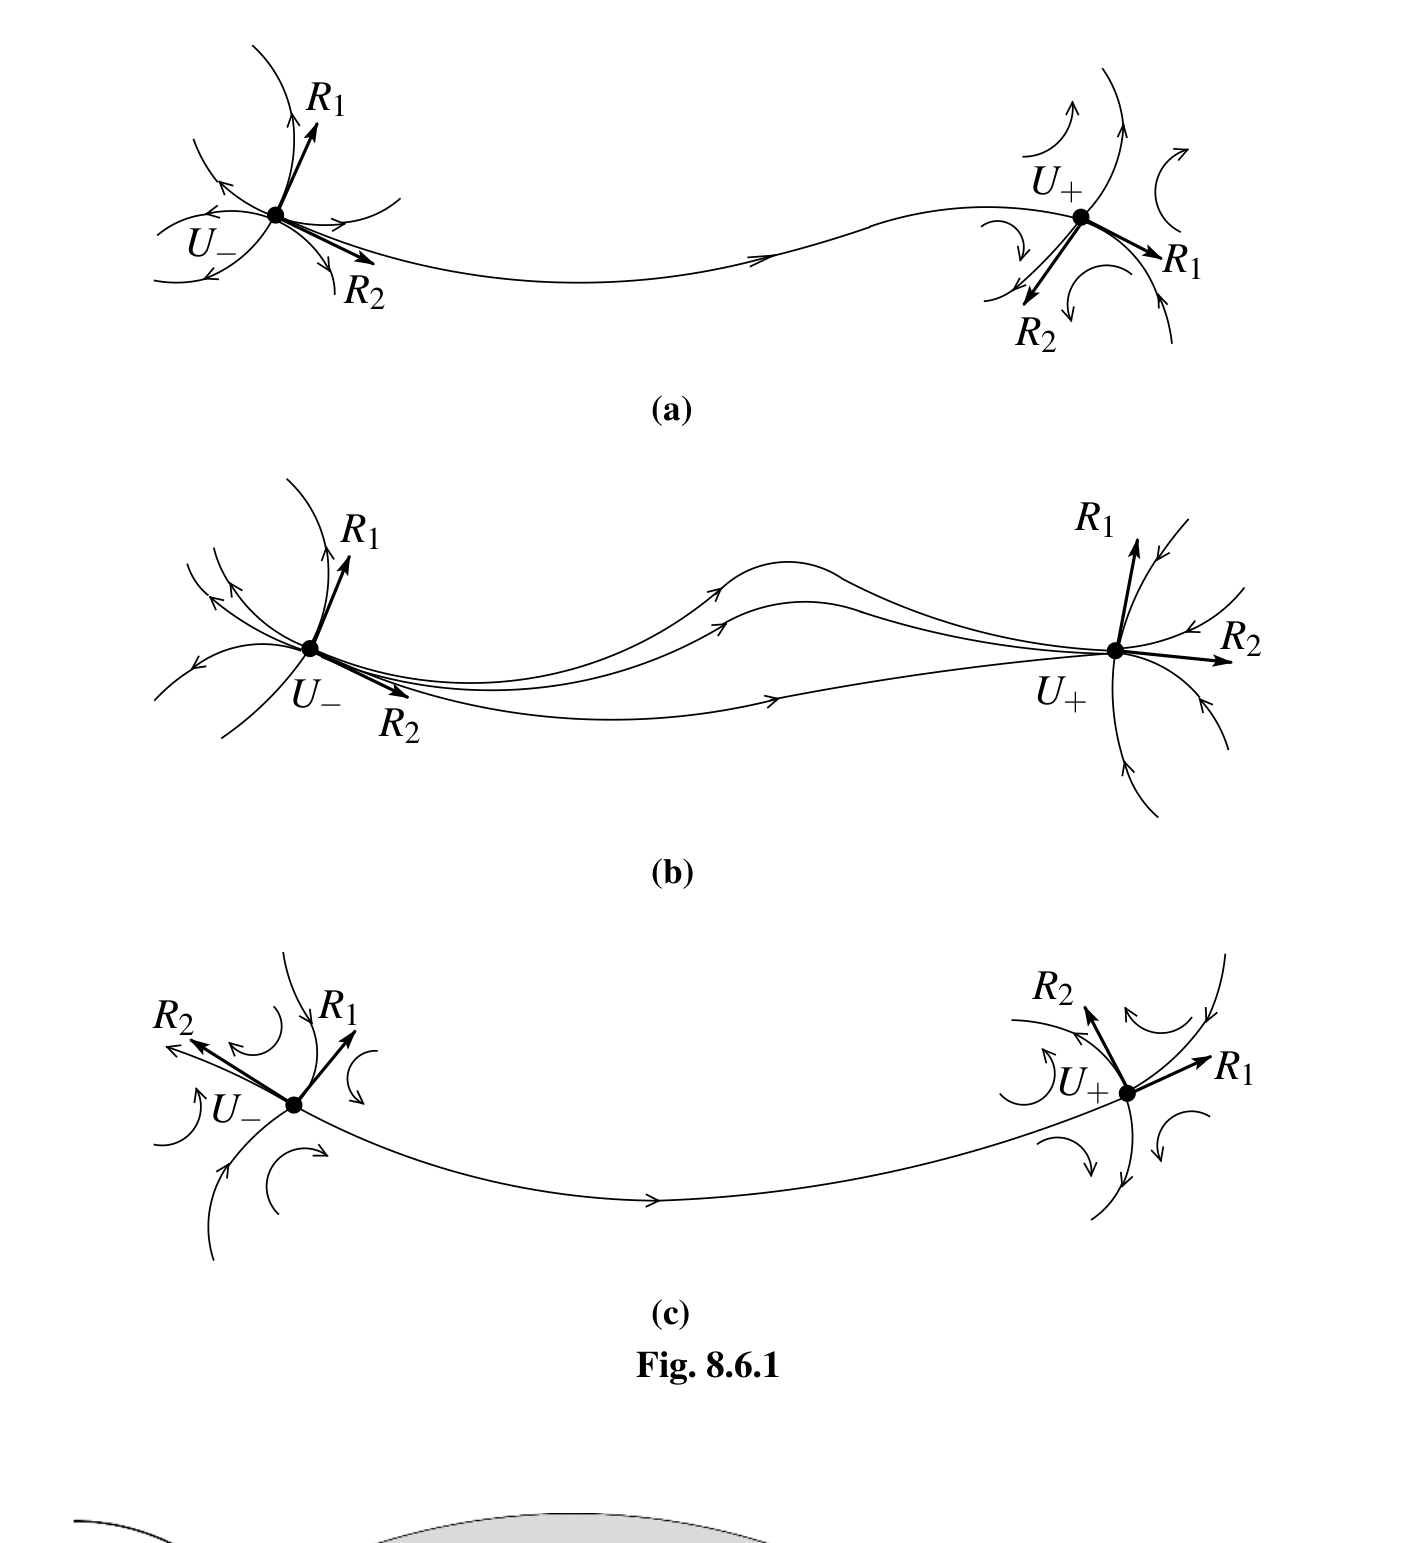
\includegraphics[width=0.78\textwidth]{ch08-fig06-01.png}
\caption{压缩、超压缩与亚压缩激波剖面的三种相图模式：(a) 压缩激波（$n=2$，$i=j=1$）；(b) 超压缩激波（$n=2$，$i=1$，$j=2$）；(c) 亚压缩激波（$n=2$，$i=2$，$j=1$）}\label{figure:ch08-三模式}
\end{figure}

\begin{figure}[ht]
\centering
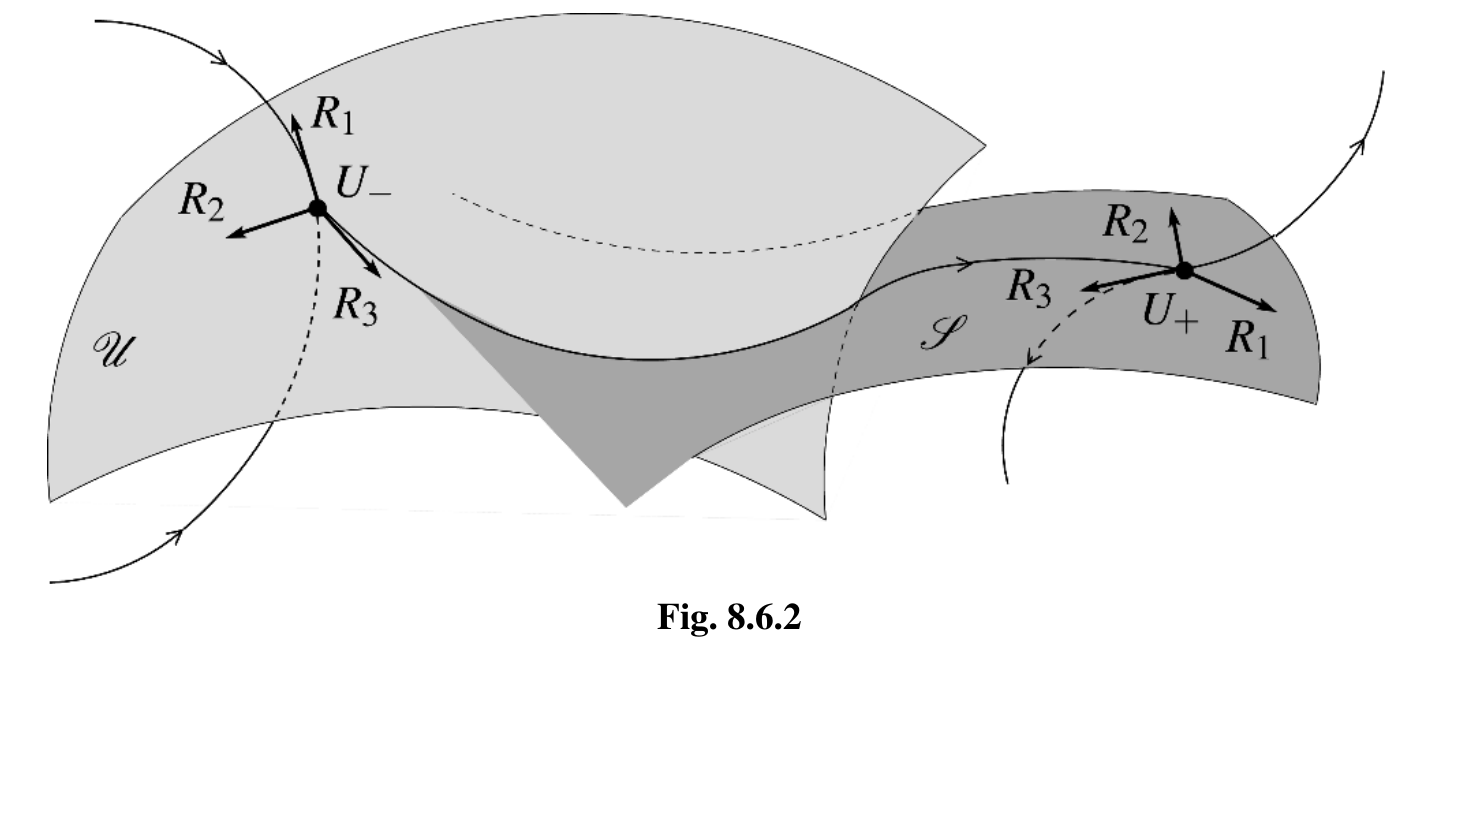
\includegraphics[width=0.78\textwidth]{ch08-fig06-02.png}
\caption{$n=3$、$i=j=2$ 时，二维不稳定流形 $\mathscr U$ 与二维稳定流形 $\mathscr S$ 横截相交，形成连接 $U_-$ 与 $U_+$ 的唯一黏性激波剖面}\label{figure:ch08-二三流形}
\end{figure}

对超压缩激波（即 $i<j$），$\dim\mathscr U+\dim\mathscr S=n+1+j-i$，故 $\mathscr U\cap\mathscr S$ 是维数为 $j-i+1\geqslant2$ 的流形。因此 $U_-$ 与 $U_+$ 由无穷多条黏性激波剖面相连。该构型也是结构稳定的。图\ref{figure:ch08-三模式} (b) 描绘了 $n=2$、$i=1$、$j=2$ 的此类模式：不稳定结点 $U_-$ 由无穷多条黏性激波剖面连接到稳定结点 $U_+$。

对亚压缩激波（即 $i>j$），$\dim\mathscr U+\dim\mathscr S<n+1$，于是一般地 $\mathscr U$ 与 $\mathscr S$ 不相交。因而一般不存在连接 $U_-$ 与 $U_+$ 的黏性激波剖面；而在它存在的非一般情形，该剖面是结构不稳定的。这见图\ref{figure:ch08-三模式} (c)：$n=2$、$i=2$、$j=1$，一条结构不稳定的黏性激波剖面连接两个鞍点 $U_-$ 与 $U_+$。

上述情形（黏性激波剖面的存在性仅取决于压缩性）出现在激波为弱激波或系统具有特殊结构时。一般而言，黏性激波剖面的存在性还依赖于激波的内部结构。为洞悉这一问题，我们先看两个简单例子，从带有相应耗散方程\eqref{align:ch08-标量黏性} 的单个守恒律\eqref{align:ch07-标量守恒律} 开始。此时\eqref{align:ch08-剖面ode} 蜕化为标量方程
\begin{align}
\dot u=f(u)-f(u_-)-s(u-u_-).
\label{align:ch08-标量剖面}
\end{align}
显然，$u_-$ 与 $u_+$ 由黏性激波剖面相连，当且仅当\eqref{align:ch08-标量剖面} 的右端在 $u_-$ 与 $u_+$ 之间不变号，且在 $u_-<u_+$ 时非负、在 $u_->u_+$ 时非正。回顾\eqref{align:ch08-扰动方程}，我们得出：在单个守恒律\eqref{align:ch07-标量守恒律} 中，激波满足黏性激波容许性准则，当且仅当 Oleinik $E$-条件\eqref{align:ch08-oleinik} 成立。当\eqref{align:ch08-oleinik} 对介于 $u_-$ 与 $u_+$ 之间（严格）的任一 $u_0$ 以严格不等式成立时，$u_-$ 与 $u_+$ 由单条轨道相连。与之相反，当\eqref{align:ch08-oleinik} 对一中间集 $u_0$ 取等号时，我们需要不止一条轨道，甚至可能需要若干接触间断，才能构造出黏性激波剖面。此时可宁可把激波可视作若干以同一速度传播的激波和/或接触间断的复合。

接下来转向系统\eqref{align:ch07-p系统} 及相应耗散系统\eqref{align:ch08-弹性黏性}。此时\eqref{align:ch08-剖面ode} 读作
\begin{align}
\begin{cases}
0=-v+v_--s(u-u_-)\\
u^{-1}\dot v=-\sigma(u)+\sigma(u_-)-s(v-v_-).
\end{cases}
\label{align:ch08-弹性剖面系统}
\end{align}
我们最终得到代数方程与微分方程的组合而非仅微分方程，其原因是 $B$ 是奇异矩阵。无论如何，在\eqref{align:ch08-弹性剖面系统} 的两个方程之间消去 $v$，推得
\begin{align}
s\,u^{-1}\dot u=\sigma(u)-\sigma(u_-)-s^2(u-u_-).
\label{align:ch08-弹性剖面}
\end{align}
由于 $u>0$，$(u_-,v_-)$ 与 $(u_+,v_+)$ 由黏性激波剖面相连，当且仅当\eqref{align:ch08-弹性剖面} 的右端在 $u_-$ 与 $u_+$ 之间不变号，且在 $s(u_+-u_-)>0$ 时非负、在 $s(u_+-u_-)<0$ 时非正。由\eqref{align:ch08-气体r}，我们得出：在等熵弹性系统\eqref{align:ch07-p系统} 中，激波满足黏性激波容许性准则，当且仅当 Wendroff $E$-条件\eqref{align:ch08-wendroff} 成立。

正是通过上述论证导出的 Oleinik $E$-条件与 Wendroff $E$-条件，为一般 Liu $E$-条件提供了动机。我们现着手证明：黏性激波容许性准则一般等价于 Liu $E$-条件，至少在中等强度激波范围内如此。为简单起见，此处仅讨论 $B=I$ 的特殊情形；更一般 $B$ 的情形见\hyperref[section:ch08-注记]{8.8 节}所引文献。

\begin{theorem}[中等强度激波：黏性准则等价于 Liu 准则]\label{theorem:ch08-黏性等价liu}
设 $\lambda_i$ 是 $\mathrm{D}F$ 的单特征值。则一个中等强度的 $i$-激波在 $B=I$ 时满足黏性激波容许性准则，当且仅当它满足 Liu $E$-条件。
\end{theorem}

\begin{proof}
设左侧状态 $U_-$ 由一个中等强度、速度为 $s$ 的 $i$-激波在右侧连接到状态 $U_+$。为施加黏性激波容许性检验，首要任务是在状态空间中构造一条连接 $U_+$ 与 $U_-$、并在\eqref{align:ch08-id剖面} 生成的流下不变的曲线。为此，我们引入一个新的（标量）变量 $r$，将\eqref{align:ch08-id剖面} 嵌入一个更大的自治系统：
\begin{align}
\begin{cases}
\dot V=F(V)-F(U_-)-r[V-U_-]\\
\dot r=0.
\end{cases}
\label{align:ch08-增广系统}
\end{align}
注意，\eqref{align:ch08-增广系统} 右端在平衡点 $V=U_-$、$r=\lambda_i(U_-)$ 处取值的 Jacobian 矩阵为
\begin{align}
J=\left(\begin{array}{c|c}
\mathrm{D}F(U_-)-\lambda_i(U_-)I&0\\ \hline 0&0
\end{array}\right),
\label{align:ch08-jacobian}
\end{align}
其特征值为 $\lambda_j(U_-)-\lambda_i(U_-)$（$j=1,\cdots,n$）及 $0$；相应特征向量为
\begin{align}
\begin{pmatrix}R_j(U_-)\\0\end{pmatrix},\quad j=1,\cdots,n,\qquad\text{以及}\qquad\begin{pmatrix}0\\1\end{pmatrix}.
\label{align:ch08-特征向量}
\end{align}
我们看到 $J$ 有两个零特征值，关联于一个二维特征空间，其余特征值为非零实数。于是中心流形定理蕴涵：任何局限在点 $(U_-,\lambda_i(U_-))$ 小邻域内的\eqref{align:ch08-增广系统} 轨道，必位于一个二维流形 $\mathscr M$ 上，它在\eqref{align:ch08-增广系统} 生成的流下不变，并可参数化为
\begin{align}
V=\Phi(\zeta,r)=U_-+\zeta R_i(U_-)+S(\zeta,r),\qquad r=r,
\label{align:ch08-中心流形}
\end{align}
其中
\begin{align}
S(0,\lambda_i(U_-))=0,\qquad S_\zeta(0,\lambda_i(U_-))=0,\qquad S_r(0,\lambda_i(U_-))=0.
\label{align:ch08-中心条件}
\end{align}
特别地，\eqref{align:ch08-增广系统} 的平衡点 $(U_+,s)$ 必位于 $\mathscr M$ 上，此时 $U_+=\Phi(\rho,s)$，其中 $\rho$ 接近 $0$。于是 $U_-$ 与 $U_+$ 由光滑曲线 $V=\Phi(\zeta,s)$（$\zeta$ 介于 $0$ 与 $\rho$ 之间）相连，且该曲线在\eqref{align:ch08-id剖面} 生成的流下不变。

沿不变曲线 $V=\Phi(\cdot,r)$，由\eqref{align:ch08-增广系统} $_1$ 诱导的流由函数 $\zeta=\zeta(\cdot)$ 表示，它满足标量常微分方程
\begin{align}
\dot\zeta=g(\zeta,r),
\label{align:ch08-gzeta}
\end{align}
其中 $g$ 定义为
\begin{align}
g(\zeta,r)\,\Phi_\zeta(\zeta,r)=F(\Phi(\zeta,r))-F(U_-)-r[\Phi(\zeta,r)-U_-].
\label{align:ch08-g定义}
\end{align}
特别地，回顾\eqref{align:ch08-中心流形} 与\eqref{align:ch08-中心条件}，
\begin{align}
g(0,r)=0,\qquad g_\zeta(0,r)=\lambda_i(U_-)-r.
\label{align:ch08-g初值}
\end{align}
显然，黏性激波容许性准则成立，当且仅当对介于 $0$ 与 $\rho$ 之间的所有 $\zeta$ 有 $\rho g(\zeta,s)\geqslant0$。

现设激波满足 Liu $E$-条件。于是，若 $W_i$ 表示过 $U_-$ 的 $i$-激波曲线、$s_i$ 为相应激波速度函数，从而 $U_-=W_i(0)$、$U_+=W_i(\tau_+)$、$s=s_i(\tau_+)$，则必有对介于 $0$ 与 $\tau_+$ 之间的 $\tau$ 有 $s_i(\tau)\geqslant s$。为确定起见，设 $U_+-U_-$ 近似指向 $R_i(U_-)$ 的方向，此时 $\rho$ 与 $\tau_+$ 均为正。

我们固定 $r<s$（$s-r$ 很小），考虑曲线 $\Phi(\cdot,r)$ 并确定 $\kappa>0$ 使 $[\Phi(\kappa,r)-U_+]^\top R_i(U_-)=0$。我们证明 $g(\zeta,r)>0$（$0<\zeta<\kappa$）。确实，若对某个 $\zeta$（$0<\zeta<\kappa$）有 $g(\zeta,r)=0$，则由\eqref{align:ch08-g定义}，状态 $\Phi(\zeta,r)$ 可由速度为 $r$ 的激波连到状态 $U_-$。于是 $\Phi(\zeta,r)$ 位于激波曲线 $W_i$ 上，记作 $\Phi(\zeta,r)=W_i(\tau)$，其中 $\tau$ 为某数。由 $\kappa$ 的构造，因 $0<\zeta<\kappa$，必有 $0<\tau<\tau_+$。然而此时 $r=s_i(\tau)\geqslant s$，与假设 $r<s$ 矛盾。这就证明了 $g(\zeta,r)$ 在 $(0,\kappa)$ 上不变号。同时，回顾\eqref{align:ch08-g初值}，$g_\zeta(0,r)=s_i(0)-r\geqslant s-r>0$，这表明 $g(\zeta,r)>0$（$0<\zeta<\kappa$）。最后令 $r\uparrow s$，此时 $\kappa\to\rho$。故对 $\zeta\in(0,\rho)$ 有 $g(\zeta,s)\geqslant0$。

由类似论证可证明逆命题：对介于 $0$ 与 $\rho$ 之间的 $\zeta$ 有 $\rho g(\zeta,s)\geqslant0$，蕴涵对介于 $0$ 与 $\tau_+$ 之间的 $\tau$ 有 $s_i(\tau)\geqslant s$。证明完毕。
\end{proof}

联立\cref{theorem:ch08-liu蕴涵lax}、\cref{theorem:ch08-真非线性等价} 与\cref{theorem:ch08-黏性等价liu}，我们得出：黏性激波容许性准则一般蕴涵 Lax $E$-条件，但逆命题一般不成立，除非系统真非线性且激波为弱激波。

应当强调，黏性激波容许性准则与 Liu $E$-条件之间的等价性一般依赖于黏性矩阵 $B$ 的选取。为看清这一点，考虑简单系统
\begin{align}
\partial_t(u,v,w)^\top+\partial_x(u^2,v^2,w^2)^\top=0,
\label{align:ch08-三个burgers}
\end{align}
它由 Burgers 方程的三个非耦合拷贝组成。在左侧连接状态 $(-3,7,-1)^\top$、在右侧连接状态 $(5,-5,3)^\top$、并以速度 $s=2$ 传播的亚压缩激波，违反 Lax $E$-条件、Liu $E$-条件，且当黏性矩阵 $B=I$ 时也违反黏性激波容许性准则。然而，对下述对称正定黏性矩阵，该激波确实满足黏性激波容许性条件：
\begin{align}
B=\begin{pmatrix}9&8&2\\8&9&2\\2&2&1\end{pmatrix}.
\label{align:ch08-非恒等黏性}
\end{align}
确实，相应黏性激波剖面由下式给出：
\begin{align}
V(\tau)=(1,1,1)^\top+\tanh(2\tau)(4,-6,2)^\top,\qquad-\infty<\tau<\infty.
\label{align:ch08-非恒等剖面}
\end{align}

我们的下一个任务是把黏性激波容许性准则与熵激波容许性准则作比较。于是设系统\eqref{align:ch08-守恒律一维} 配有满足\eqref{align:ch07-熵流对定义}（$\mathrm{D}q=\mathrm{D}\eta\,\mathrm{D}F$）的熵--熵流对 $(\eta,q)$。熵与黏性矩阵 $B$ 之间的自然相容条件已在\cref{section:ch04-消失黏性方法}中讨论过。我们在当下一维设定中写出条件\eqref{align:ch04-黏性弱形式} 的（较弱）形式：
\begin{align}
H^\top\mathrm{D}^2\eta(U)B(U)H\geqslant0,\qquad H\in\mathbb R^n,\ U\in\mathcal O.
\label{align:ch08-熵黏性相容}
\end{align}
如\cref{section:ch04-消失黏性方法}已指出，当 $B=I$ 时，\eqref{align:ch08-熵黏性相容} 成立当且仅当 $\eta$ 为凸。

\begin{theorem}[黏性准则蕴涵熵准则]\label{theorem:ch08-黏性蕴涵熵}
当\eqref{align:ch08-熵黏性相容} 成立时，任一满足黏性激波容许性准则的激波也满足熵激波容许性准则。
\end{theorem}

\begin{proof}
考虑一个速度为 $s$、在左侧连接状态 $U_-$、在右侧连接状态 $U_+$、并满足黏性激波容许性条件的激波。

首先设 $U_-$ 与 $U_+$ 由\eqref{align:ch08-剖面ode} 的单条轨道相连，即存在函数 $V$ 在 $(-\infty,\infty)$ 上满足\eqref{align:ch08-剖面ode}，从而也满足\eqref{align:ch08-行波ode}，并满足 $V(\tau)\to U_\pm$（$\tau\to\pm\infty$）。从左侧以 $\mathrm{D}\eta(V(\tau))$ 乘以\eqref{align:ch08-行波ode} 并使用\eqref{align:ch07-熵流对定义}，得
\begin{align}
\big[\mathrm{D}\eta(V)B(V)\dot V\big]^{\cdot}-\dot V^\top\mathrm{D}^2\eta(V)B(V)\dot V=\dot q(V)-s\dot\eta(V).
\label{align:ch08-熵积分}
\end{align}
在 $(-\infty,\infty)$ 上积分\eqref{align:ch08-熵积分} 并使用\eqref{align:ch08-熵黏性相容}，便得到\eqref{align:ch08-熵条件}。我们由此证明了激波满足熵条件。

在黏性激波剖面含有中间平衡点的一般情形，我们把激波实现为有限或无穷多个上述类型简单激波和/或接触间断的复合，它们都以同一速度 $s$ 传播。如上所示，跨过每条简单激波的熵产生非正。另一方面，由\cref{theorem:ch08-接触熵零}，跨过任一接触间断的熵产生为零。因此，合并各部分熵产生，得出总熵产生\eqref{align:ch08-熵条件} 非正。证明完毕。
\end{proof}

\cref{theorem:ch08-黏性蕴涵熵} 的逆命题一般不成立。例如考虑等熵弹性系统\eqref{align:ch07-p系统}、相应耗散系统\eqref{align:ch08-弹性黏性} 及熵--熵流对\eqref{align:ch07-p系统熵}，它们满足相容条件\eqref{align:ch08-熵黏性相容}。如\hyperref[section:ch08-熵激波容许性准则]{8.5 节}所示，熵激波容许性准则通过不等式\eqref{align:ch08-弹性熵条件} 检验，后者由 Wendroff $E$-条件\eqref{align:ch08-wendroff} 导出，但一般不被其蕴涵。

为稳健起见，黏性方法应当把激波\eqref{align:ch08-间断} 生成作\eqref{align:ch08-黏性方程} 的解（作为相应黏性激波剖面\eqref{align:ch08-行波形式} 的扰动）当 $\mu\downarrow0$ 时的极限。对固定的 $t$，令 $\mu\downarrow0$ 等价于通过坐标伸缩对固定 $\mu$ 令 $t\to\infty$。于是可以有理由地论证：用来检验激波容许性的黏性激波剖面，必须源自\eqref{align:ch08-黏性方程} 的渐近稳定行波解。这一问题近年来已被透彻研究，并已形成一套完整理论，足以撰写专著。详尽论述超出本书范围，此处仅报告要点。细节与证明见\hyperref[section:ch08-注记]{8.8 节}所引文献。

为简单起见，我们把讨论限于黏性矩阵 $B=I$，并通过置 $\mu=1$ 规范化\eqref{align:ch08-黏性方程}。考虑一个弱 $i$-激波，在左侧连接状态 $U_-$、在右侧连接状态 $U_+$，它允许一条黏性激波剖面 $V$。变换变量 $x\mapsto x+st$ 使激波定常。黏性激波剖面 $V$ 称为\emph{渐近稳定的}，如果以 $U(x,0)=V(x)+U_0(x)$ 为初值（其中 $U_0$ 是在 $\pm\infty$ 衰减的“小”扰动）的\eqref{align:ch08-黏性方程} 解 $U(x,t)$ 满足
\begin{align}
U(x,t)\to V(x+h),\qquad t\to\infty,
\label{align:ch08-渐近稳定}
\end{align}
其中 $h\in\mathbb R$ 为某个适当的相移。

由\eqref{align:ch08-黏性方程} 解的总质量守恒这一观察所驱动，自然要求\eqref{align:ch08-渐近稳定} 中的收敛在 $L^1(-\infty,\infty)$ 中。特别地，这将意味着 $V(x+h)$ 携带扰动引入的过剩质量：
\begin{align}
\int_{-\infty}^{\infty}U_0(x)\,\mathrm{d}x=\int_{-\infty}^{\infty}\big[V(x+h)-V(x)\big]\,\mathrm{d}x=h[U_+-U_-].
\label{align:ch08-质量}
\end{align}
在标量情形 $n=1$，对任意扰动 $U_0\in L^1(-\infty,\infty)$，任一黏性激波剖面在 $L^1(-\infty,\infty)$ 中渐近稳定，其中 $h$ 由\eqref{align:ch08-质量} 确定。

对系统 $n\geqslant2$，单个标量参数 $h$ 一般不足以平衡向量方程\eqref{align:ch08-质量}，此时\eqref{align:ch08-渐近稳定} 不能在 $L^1(-\infty,\infty)$ 中成立，因为单靠 $V$ 的 $h$-平移无法携带过剩质量。对\eqref{align:ch08-黏性方程} 渐近性的深刻分析表明，对大 $t$，解 $U$ 应发展出一条黏性激波剖面，并伴以一族所谓扩散波，它们分担携带质量的负担：
\begin{align}
U(x,t)\sim V(x+h)+W(x,t)+\sum_{j<i}\theta_j(x,t)R_j(U_-)+\sum_{j>i}\theta_j(x,t)R_j(U_+).
\label{align:ch08-渐近展开}
\end{align}
\eqref{align:ch08-渐近展开} 右端求和中的 $j$ 项表示一个\emph{解耦的 $j$-扩散波}。标量函数 $\theta_j$ 是非线性扩散方程
\begin{align}
\partial_t\theta_j+\partial_x\Big[\lambda_j\theta_j+\tfrac12(\mathrm{D}\lambda_j R_j)\theta_j^2\Big]=\partial_x^2\theta_j
\label{align:ch08-扩散方程}
\end{align}
的自相似解
\begin{align}
\theta_j(x,t)=\frac{1}{\sqrt t}\,\phi_j\!\left(\frac{x-\lambda_j t}{\sqrt t}\right).
\label{align:ch08-扩散波}
\end{align}
在\eqref{align:ch08-扩散波}、\eqref{align:ch08-扩散方程} 中，$\lambda_j$、$\mathrm{D}\lambda_j$、$R_j$ 对 $j=1,\cdots,i-1$ 在 $U_-$ 处取值，对 $j=i+1,\cdots,n$ 在 $U_+$ 处取值。于是 $j$-扩散波具有钟形剖面，以特征速度 $\lambda_j$ 传播；其峰值以 $O(t^{-1/2})$ 衰减，而质量保持常数，记作 $m_j R_j$。\eqref{align:ch08-渐近展开} 右端剩余项 $W$ 表示\emph{耦合扩散波}，它满足一个复杂的线性扩散方程，与解耦扩散波以相同速率衰减，但不携带质量。因此，当 $t\to\infty$ 时的质量守恒给出替代\eqref{align:ch08-质量} 的方程
\begin{align}
\int_{-\infty}^{\infty}U_0(x)\,\mathrm{d}x=\sum_{j<i}m_jR_j(U_-)+h[U_+-U_-]+\sum_{j>i}m_jR_j(U_+),
\label{align:ch08-质量分配}
\end{align}
它规定了过剩质量如何在黏性激波剖面与解耦扩散波之间分配。由于 $U_+-U_-$ 与 $R_i(U_\pm)$ 近似共线，\eqref{align:ch08-质量分配} 显式且唯一地确定黏性激波剖面的相移 $h$ 以及各 $j$-扩散波的质量 $m_j$。

已证：对 $V$ 的任一满足
\begin{align}
\int_{-\infty}^{\infty}(1+x^2)|U_0(x)|^2\,\mathrm{d}x\ll1
\label{align:ch08-小扰动}
\end{align}
的扰动 $U_0\in H^1(-\infty,\infty)$，由\eqref{align:ch08-质量分配} 确定的 $h$，黏性激波剖面 $V$ 在 $L^\infty(-\infty,\infty)$ 中渐近稳定\eqref{align:ch08-渐近稳定}，只要特征值 $\lambda_i$ 为单且激波满足严格形式的 Lax $E$-条件。应当指出，即使 $i$-特征族非真非线性，这一断言仍成立。

上述井然结构在处理超压缩或亚压缩激波时瓦解，偶尔在强压缩激波时亦然。为一瞥此类情形可能出现的几何复杂性，我们讨论简单系统\eqref{align:ch07-脐点模型}（耗散形式\eqref{align:ch08-模型黏性}）的 2-激波的黏性激波剖面构造。激波性质已在\hyperref[section:ch08-lax容许性准则]{8.3 节}中讨论过。利用系统在旋转下的对称性与伸缩性质，我们不失一般性地把左侧状态 $(u_-,v_-)$ 固定在点 $(1,0)$。右侧状态 $(u_+,v_+)$ 将位于点 $(a,0)$，其中 $a\in(-\frac12,0)$。此时，如\hyperref[section:ch08-lax容许性准则]{8.3 节}所示，激波速度为 $s=a^2+a+1$，激波是超压缩的\eqref{align:ch08-lax-e}。注意状态 $(b,0)$（其中 $b=-1-a$）也由同一速度 $s$ 的 2-激波连到 $(1,0)$，该激波满足 Lax $E$-条件且非超压缩，但不满足 Liu $E$-条件。

关联于\eqref{align:ch08-模型黏性} 的系统\eqref{align:ch08-剖面ode} 读作：
\begin{align}
\begin{cases}
\dot u=-s(u-1)+u(u^2+v^2)-1\\
\dot v=-sv+v(u^2+v^2);
\end{cases}
\label{align:ch08-模型剖面}
\end{align}
或等价地，在极坐标 $(\rho,\theta)$（$u=\rho\cos\theta$，$v=\rho\sin\theta$）中：
\begin{align}
\begin{cases}
\dot\rho=\rho(\rho^2-s)+(s-1)\cos\theta\\
\rho\dot\theta=-(s-1)\sin\theta.
\end{cases}
\label{align:ch08-极坐标剖面}
\end{align}

注意\eqref{align:ch08-模型剖面} 有三个平衡点：(a) $(1,0)$，是不稳定结点；(b) $(a,0)$，是稳定结点；(c) $(b,0)$，是鞍点。通过对\eqref{align:ch08-模型剖面} 与\eqref{align:ch08-极坐标剖面} 的初等分析容易确定的相图，绘于图\ref{figure:ch08-模型相图}。

\begin{figure}[ht]
\centering
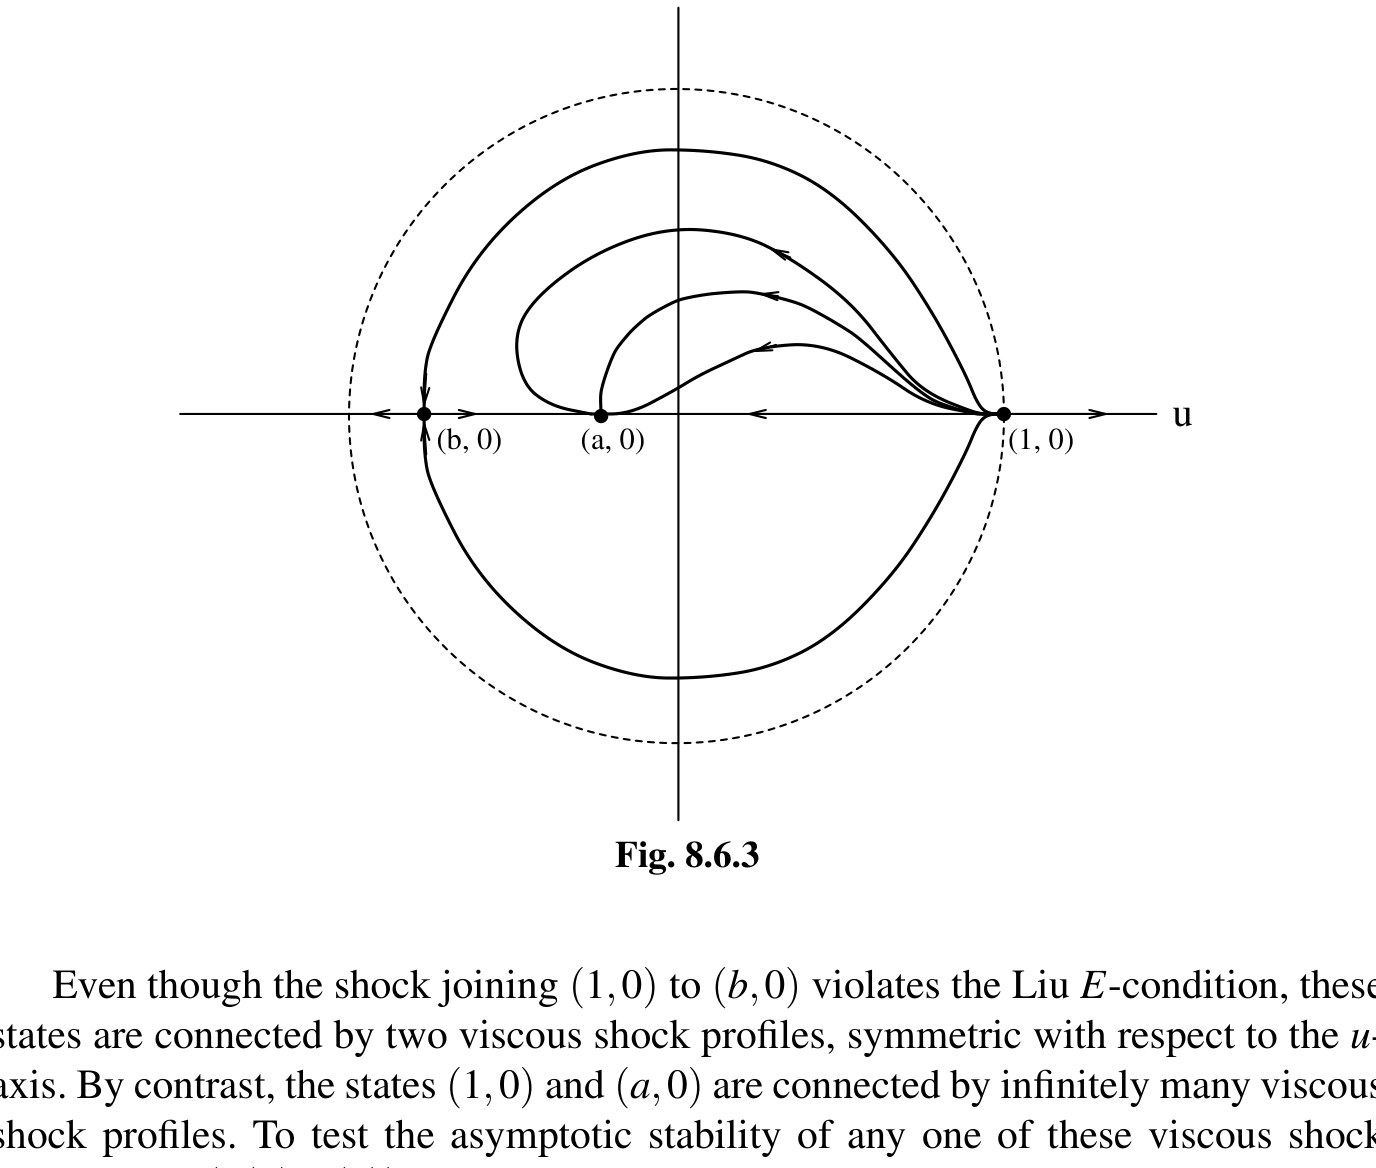
\includegraphics[width=0.62\textwidth]{ch08-fig06-03.png}
\caption{系统\eqref{align:ch08-模型剖面} 的相图：空心虚线圆为圆周 $u^2+v^2=1$；实心点依次为不稳定结点 $(1,0)$、稳定结点 $(a,0)$ 与鞍点 $(b,0)$}\label{figure:ch08-模型相图}
\end{figure}

尽管连接 $(1,0)$ 与 $(b,0)$ 的激波违反 Liu $E$-条件，这两个状态由关于 $u$ 轴对称的两条黏性激波剖面相连。与之相反，状态 $(1,0)$ 与 $(a,0)$ 由无穷多条黏性激波剖面相连。为检验其中任一条黏性激波剖面（记作 $(\bar u(\tau),\bar v(\tau))$）的渐近稳定性，根据上面的讨论，我们引入小扰动 $(u_0(x),v_0(x))$，并询问以
\begin{align}
(u,v)(x,0)=\left(\bar u\!\left(\frac{x}{\mu}\right)+u_0(x),\ \bar v\!\left(\frac{x}{\mu}\right)+v_0(x)\right)
\label{align:ch08-模型初值}
\end{align}
为初值的\eqref{align:ch08-模型黏性} 解 $(u,v)(x,t)$ 是否满足
\begin{align}
(u,v)(x,t)\to\left(\hat u\!\left(\frac{x-st}{\mu}\right),\ \hat v\!\left(\frac{x-st}{\mu}\right)\right),\qquad t\to\infty,
\label{align:ch08-模型收敛}
\end{align}
其中 $(\hat u(\tau),\hat v(\tau))$ 是一条（一般不同的）黏性激波剖面。由于此处不可能有扩散波，\eqref{align:ch08-模型收敛} 中的收敛必须在 $L^1(-\infty,\infty)$ 中。特别地，过剩质量守恒的 $v$-分量给出
\begin{align}
\int_{-\infty}^{\infty}v_0(x)\,\mathrm{d}x
=\int_{-\infty}^{\infty}\left[\hat v\!\left(\frac{x-st}{\mu}\right)-\bar v\!\left(\frac{x-st}{\mu}\right)\right]\mathrm{d}x
=\mu\int_{-\infty}^{\infty}\big[\hat v(\tau)-\bar v(\tau)\big]\,\mathrm{d}\tau.
\label{align:ch08-模型质量}
\end{align}
可以证明，\eqref{align:ch08-模型质量} 右端的积分一致有界，与 $\bar v$、$\hat v$ 的选取无关。因此，当 $v_0$ 固定使 $\int v_0\,\mathrm{d}x\neq0$ 时，对充分小的 $\mu$，\eqref{align:ch08-模型质量} 不能成立。于是，就激波容许性取决于连接激波剖面的稳定性而言，系统\eqref{align:ch07-脐点模型} 的超压缩激波应被称为不容许的。

近年来已出现一套非常技术性的多空间维黏性激波剖面线性稳定性理论，与\hyperref[section:ch08-lax容许性准则]{8.3 节}末扼要勾勒的多空间维激波相应理论相平行。论述见\hyperref[section:ch08-注记]{8.8 节}所引文献。

如\cref{section:ch04-消失黏性方法}所指出，在某些情形，物理相关的容许性条件不是由黏性准则、而是由黏性--毛细准则提供，此时\eqref{align:ch08-黏性方程} 由下式代替：
\begin{align}
\partial_t U(x,t)+\partial_x F(U(x,t))
=\mu\,\partial_x\big[B(U(x,t))\partial_x U(x,t)\big]
+\nu\,\partial_x\big[H(U(x,t))\partial_x^2 U(x,t)\big].
\label{align:ch08-黏性毛细}
\end{align}
一般地，当 $\nu=o(\mu^2)$ 时扩散主导，而当 $\mu=o(\sqrt\nu)$ 时色散占优。当 $\nu=\mu^2$ 时两种效应平衡。此时激波剖面由常微分方程
\begin{align}
H(V)\ddot V+B(V)\dot V=F(V)-F(U_-)-s[V-U_-]
\label{align:ch08-毛细剖面}
\end{align}
控制，以代替\eqref{align:ch08-剖面ode}。此类剖面的理论正在文献中逐渐形成。

\end{document}
